\documentclass[10pt,twocolumn]{exam}
\usepackage[hon]{template-for-exam}
\usepackage{endnotes,graphicx}
\usepackage{tikz,tikzpingus,graphicx,enumitem,stfloats}
\graphicspath{{./figures/}}
%\pinguloadlibrary{horse}
\usetikzlibrary{shadings,decorations.pathmorphing,arrows.meta,patterns}
\def\answer#1{\footnotetext{#1}}
\def\theanswers{\theendnotes}
\def\myquestion{\question\stepcounter{footnote}}
%\def\enoteheading{Answer}

\title{Chapter 3 Homework}
\author{Rohrbach}
\date{\today}

\begin{document}
\maketitle




\noindent
\textit{Questions and figures are from OpenStax} College Physics \textit{2nd ed (Chapter 3) or Giancolli} Physics: Principles with Applications \textit{7th ed. (Chapter 3) unless otherwise noted.}

\section*{3.2 Graphical Methods}

\begin{questions}

 
\uplevel{
  \subsection*{Problems}
}
  
\myquestion (OpenStax P1, modified)
Find the following for path A in Figure~\ref{3-49}. (All blocks are 120 m on a side.)

\begin{parts} \answer{(b) 480 m; (d) $\approx 380$ m @ $20^\circ$ E of N}
  \part Draw the path to scale on your paper. (You can either use a scale like 1 cm = 1 block or 1 square of graph paper = 1 block)
  \part Determine the distance traveled.
  \part Use your ruler to draw the displacement vector from start to finish.
  \part Measure the magnitude of the displacement vector and estimate its direction.
\end{parts}


\begin{figure*}[b]
  \centering
  \includegraphics[height=2.5in]{3-49.jpg}
  \caption{(OpenStax Fig 3.49) The various lines represent paths taken by different people walking in a city. All blocks are 120 m on a side.}
  \label{3-49}
\end{figure*}

\myquestion (OpenStax P2, modified) Repeat problem 1 for path B in Figure~\ref{3-49}. \answer{(b) 1200 m; (d) $\approx 380$ m @ $20^\circ$ E of N}

\myquestion (OpenStax P13, modified) Repeat problem 1 for path C in Figure~\ref{3-49}. \answer{(b) 1560 m; (d) 120 m east}

\pagebreak 

\vspace*{\stretch{1}}
\uplevel{\subsection*{Conceptual Questions}}

\begin{enumerate}[label=CQ\arabic*.]
  \item (OpenStax CQ1) Which of the following is a vector: a person's height, the altitude on Mt. Everest, the age of the Earth, the boiling point of water, the cost of this book, the Earth's population, the acceleration of gravity?
  \item (OpenStax CQ3)  What do vectors \& scalars have in common? How do they differ?
  \item (Giancolli CQ1) One car travels due east at 40~km/h, and a second car traveks north at 40~km/h.  Are their velocities equal? Explain.
  \item (Giancolli CQ4) Can the displacement vector for a particle moving in two dimensions be longer than the length of the path traveled by the particle over the same time interval? Can it be less? Discuss.
\end{enumerate}


\pagebreak
\uplevel{\section*{3.3 Analytical Methods}}

\uplevel{\subsection*{Problems}}

\myquestion \label{SanFran} (OpenStax P15) Find the north and east components of the displacement from San Francisco to Sacramento shown in Figure~\ref{3-54}. \answer{$S_x=S_y=\SI{87.0}{km}$}

  \begin{figure}[ht]
    \centering
    \includegraphics[width=2in]{3-54.jpg}
    \caption{(OpenStax Fig~3.54) For problem \#\ref{SanFran}.}
    \label{3-54}
  \end{figure}

\myquestion (OpenStax P16) \hfill Suppose you walk 18.0 m straight west and then 25.0 m straight north. How far are you from your starting point, and what is the compass direction of a line connecting your starting point to your final position?  (If you represent the two legs of the walk as vector displacements $\vec{A}$ and $\vec{B}$, as in Figure~\ref{3-55}, then this problem asks you to find their sum $\vec{R}=\vec{A}+\vec{B}$.) \answer{30.8 m @ 35.8$^\circ$ W of N}

  \begin{figure}[h]
    \centering
    \includegraphics[width=2.2in]{3-55.jpg}
    \caption{(OpenStax Fig 3.55) The two displacements $\vec{A}$ and $\vec{B}$ add to give a total displacement $\vec{R}$ having magnitude $R$ and direction $\theta$.}
    \label{3-55}
  \end{figure}

  \pagebreak
  

\myquestion (OpenStax P18) You drive 7.50~km in a straight line in a direction $15^\circ$ east of north. Find the distances you would have to drive straight east and then straight north to arrive at the same point. (This determination is equivalent to find the components of the displacement along the east and north directions.) \answer{$R_x = 1.94$~km; $R_y = 7.24$~km}

\myquestion (Giancolli P6) Vector $\vec{V}_1$ is 6.6 units long and points due west.  Vector $\vec{V}_2$ is 8.5 untis long and points $55^\circ$ north of east.  (a) What are the $x$- and $y$- components of each vector?  (b) Determine the sum $\vec{V}_1+\vec{V}_2$ (magnitude and angle). \answer{$v_{1x} = -6.6$, $v_{1y} = 0$; $v_{2x} = 4.88$, $v_{2y} = 6.96$; 7.17 units @ 76.1$^\circ$ N of W}

\myquestion (Giancolli P9, P10, P12) Three vectors are shown in Figure~\ref{3-35}.  Their magnitudes are given in arbitrary units. \answer{(b) $R_x = 24.0$, $R_y = 11.7$, $\vec{R} = 26.7$ units @ 26$^\circ$ N of E; (c) 53.6 units @ 1.4$^\circ$ N of W; (d) 137.2 @ 73.0$^\circ$ W of S}

\begin{parts}
  \part Calculate the components of each vector.
  \part Draw and calculate $\vec{A}+\vec{B}+\vec{C}$ (magnitude and direction).
  \part Draw and calculate $\vec{B}-\vec{A}$ (magnitude and direction).
  \part Draw and calculate $\vec{B}-3\vec{A}$  (magnitude and direction).
\end{parts}

  \begin{figure}[ht]
    \centering
    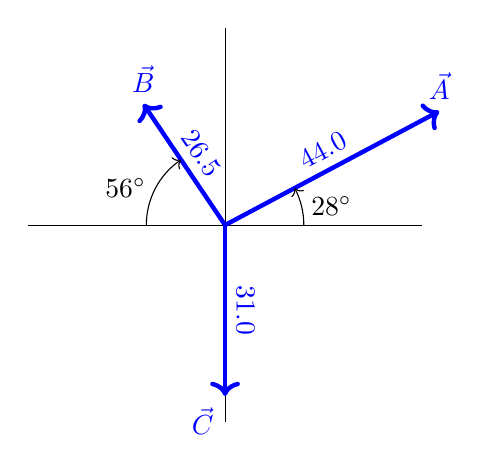
\begin{tikzpicture}
      \def\scale{0.07}
      \draw (-2.5,0) -- (2.5,0);
      \draw (0,2.5) -- (0,-2.5);
      \draw[blue, ultra thick, ->] (0,0) -- (28:44*\scale) 
        node[anchor=south] {$\vec{A}$} node[midway,sloped,above] {$44.0$};
      \draw[->] (0:1) arc (0:28:1) node[midway,anchor=west] {$28^\circ$};
      \draw[blue, ultra thick, ->] (0,0) -- (124:26.5*\scale)
        node[anchor=south] {$\vec{B}$} node[midway,sloped,above] {$26.5$};
      \draw[->] (-1,0) arc (180:124:1) node[midway,anchor=east] {$56^\circ$};
      \draw[blue, ultra thick, ->] (0,0) -- (0,-31*\scale) 
        node[anchor=north east] {$\vec{C}$} node[midway,sloped,above] {$31.0$};

    \end{tikzpicture}
    \caption{Vector magnitudes are given in arbitrary units.}
    \label{3-35}
  \end{figure}

\myquestion \textbf{Bonus!} (OpenStax P23) In an attempt to escape his island, Gilligan builds a raft and sets to sea. The wind shifts a great deal during the day, and he is blown along the following straight lines: 2.50~km  $45.0^\circ$ north of west; then 4.70~km  $60.0^\circ$ south of east; then 1.30~km $25.0^\circ$ south of west; then 5.10~km  straight east; then 1.70~km  $5.00^\circ$ east of north; then 7.20~km  $55.0^\circ$ south of west; and finally 2.80~km  $10.0^\circ$ north of east. What is his final position relative to the island?

\uplevel{
  \subsection*{Conceptual Questions}
  }

\begin{enumerate}[resume*]
  \item (OpenStax CQ9) Suppose you add two vectors $\vec{A}$ and $\vec{B}$. What relative direction between them produces the resultant with the greatest magnitude? What is the maximum magnitude? What relative direction between them produces the resultant with the smallest magnitude? What is the minimum magnitude?
  \item (OpenStax CQ10) Give an example of a nonzero vector that has a component of zero.
  \item (OpenStax CQ11) Explain why a vector cannot have a component greater than its own magnitude.
  \item (Giancolli CQ6) If $\vec{V}=\vec{V}_1+\vec{V}_2$, is $V$ necessarily greater than $V_1$ and/or $V-2$?  Discuss
\end{enumerate}



\uplevel{
  \section*{3.4   Projectile Motion (Part I)}
  \subsection*{Problems}
  }

\myquestion (OpenStax P25) \hfill
A projectile is launched at ground level with an initial speed of 50.0~m/s at an angle of $30.0^\circ$ above the horizontal. It strikes a target above the ground 3.00 seconds later. What are the $x$ and $y$ distances from where the projectile was launched to where it lands? \answer{$x=\SI{1.30e2}{m}$; $y=\SI{30.9}{m}$}

\myquestion (OpenStax P26)
A ball is kicked with an initial velocity of 16 m/s in the horizontal direction and 12 m/s in the vertical direction. (a) At what speed does the ball hit the ground? (b) For how long does the ball remain in the air? (c)What maximum height is attained by the ball? \answer{(a) 20 m/s; (b) 2.45 s; (c) 7.35 m}

\vs \pagebreak

\myquestion (OpenStax P27)
A ball is thrown horizontally from the top of a 60.0-m building and lands 100.0 m from the base of the building. Ignore air resistance. (a) How long is the ball in the air? (b) What must have been the initial horizontal component of the velocity? (c) What is the vertical component of the velocity just before the ball hits the ground? (d) What is the velocity (including both the horizontal and vertical components) of the ball just before it hits the ground?
\answer{(a) 3.50 s; (b) 28.6 m/s; (c) 34.3 m/s; (d) 44.7 m/s @ 50.2$^\circ$ below horizontal}

\myquestion (OpenStax P40)
An eagle is flying horizontally at a speed of 3.00 m/s when the fish in her talons wiggles loose and falls into the lake 5.00 m below. Calculate the velocity of the fish relative to the water when it hits the water. \answer{10.3~m/s @ 73.1$^\circ$ below horiz}

\uplevel{
  \section*{3.4   Projectile Motion (Part II)}
  \subsection*{Problems}
  }


\myquestion (OpenStax P28) 
(a) A daredevil is attempting to jump his motorcycle over a line of buses parked end to end by driving up a $32^\circ$  ramp at a speed of 40.0~m/s. How many buses can he clear if the top of the takeoff ramp is at the same height as the bus tops and the buses are 20.0~m long? (b) Discuss what your answer implies about the margin of error in this act—that is, consider how much greater the range is than the horizontal distance he must travel to miss the end of the last bus. (Neglect air resistance.)

\myquestion (OpenStax P29)
An archer shoots an arrow at a 75.0~m distant target; the bull's-eye of the target is at same height as the release height of the arrow. (a) At what angle must the arrow be released to hit the bull's-eye if its initial speed is 35.0~m/s? In this part of the problem, explicitly show how you follow the steps involved in solving projectile motion problems. (b) There is a large tree halfway between the archer and the target with an overhanging horizontal branch 3.50~m above the release height of the arrow. Will the arrow go over or under the branch?

\vs \pagebreak

\myquestion (OpenStax P33)
The cannon on a battleship can fire a shell a maximum distance of 32.0~km. (a) Calculate the initial velocity of the shell. (b) What maximum height does it reach? (At its highest, the shell is above 60\% of the atmosphere—but air resistance is not really negligible as assumed to make this problem easier.) \answer{(a) 560 m/s; (b) 8000 m} 

\myquestion (OpenStax P34)
An arrow is shot from a height of 1.5 m toward a cliff of height $H$. It is shot with a velocity of 30~m/s at an angle of $60^\circ$ above the horizontal. It lands on the top edge of the cliff 4.0~s later. (a) What is the height of the cliff? (b) What is the maximum height reached by the arrow along its trajectory? (c) What is the arrow's impact speed just before hitting the cliff?
\answer{(a) 27.0 m; (b) 13.2 m/s (c) 20 m/s}

\myquestion (OpenStax P41)
An owl is carrying a mouse to the chicks in its nest. Its position at that time is 4.00 m west and 12.0 m above the center of the 30.0 cm diameter nest. The owl is flying east at 3.50 m/s at an angle 30.0º below the horizontal when it accidentally drops the mouse. Is the owl lucky enough to have the mouse hit the nest? To answer this question, calculate the horizontal position of the mouse when it has fallen 12.0 m. \answer{4.23 m forward of drop location; misses the nest}

% \myquestion (OpenStax P43)
% Can a goalkeeper at her/ his goal kick a soccer ball into the opponent's goal without the ball touching the ground? The distance will be about 95 m. A goalkeeper can give the ball a speed of 30 m/s. \answer{No. Max range $\approx 92$ m}

\myquestion (OpenStax P45) 
In 2007, Michael Carter (U.S.) set a world record in the shot put with a throw of 24.77~m. What was the initial speed of the shot if he released it at a height of 2.10~m and threw it at an angle of $38.0^\circ$ above the horizontal? (Although the maximum distance for a projectile on level ground is achieved at $45^\circ$  when air resistance is neglected, the actual angle to achieve maximum range is smaller; thus, "38º"  will give a longer range than $45^\circ$ in the shot put.) \answer{15.0 m/s}

\myquestion \textbf{Bonus!} (OpenStax P35)
In the standing broad jump, one squats and then pushes off with the legs to see how far one can jump. Suppose the extension of the legs from the crouch position is 0.600 m and the acceleration achieved from this position is 1.25 times the acceleration due to gravity, g. How far can they jump? State your assumptions. (Increased range can be achieved by swinging the arms in the direction of the jump.) \answer{1.50 m}

\myquestion \textbf{Bonus!} (OpenStax P47)
A football player punts the ball at a $45.0^\circ$ angle. Without an effect from the wind, the ball would travel 60.0~m horizontally. (a) What is the initial speed of the ball? (b) When the ball is near its maximum height it experiences a brief gust of wind that reduces its horizontal velocity by 1.50 m/s. What distance does the ball travel horizontally?

\uplevel{
  \subsection*{Conceptual Questions}
  }

\begin{enumerate}[resume*]
  \item (Original question) When (if ever) is the velocity of a projectile fired at an angle zero?
  \item (OpenStax CQ15) For a fixed initial speed, the range of a projectile is determined by the angle at which it is fired. For all but the maximum, there are two angles that give the same range. Considering factors that F affect the ability of an archer to hit a target, such as wind, explain why the smaller angle (closer to the horizontal) is preferable. When would it be necessary for the archer to use the larger angle? Why does the punter in a football game use the higher trajectory?
  \item (Giancolli CQ15) A projectile is launched at an upward angle of $30^\circ$ to the horizontal with a speed of 30~m/s.  HOw does the horizontal component of its velocity 1.0~s after launch compare with ts horizontal component of velocity 2.0~s after launch, ignoring air resistance?  Explain.
\end{enumerate}


\uplevel{
  \section*{3.5 Addition of Velocities}
  \subsection*{Problems}
  }


\myquestion (Giancolli P38) 
A jogger is exercising on the deck of a cruise ship. The ship moves forward at a constant speed of 8.5 m/s relative to the water.
\begin{parts}
  \part While running toward the bow (front) of the ship, the jogger's speed relative to the ship is 2.0 m/s. Determine the jogger's velocity relative to the water.
  \part Later, the jogger runs toward the stern (rear) of the ship at the same speed relative to the ship. What is the jogger's velocity relative to the water in this case?
\end{parts}
\answer{(a) 10.5 m/s; (b) 6.5 m/s}

\myquestion (Giancolli P41, modified) 
 Two planes approach each other head on.  Each has a speed of 200 m/s, and they spot each other when they are initially 10 km apart.  How much time to the airplanes have to take evasive action?
 \answer{25 s}

\myquestion (OpenStax P57) 
A ship sets sail from Rotterdam, The Netherlands, heading due north at 7.00 m/s relative to the water. The local ocean current is 1.50 m/s in a direction $40.0^\circ$  north of east. What is the velocity of the ship relative to the Earth?

\myquestion \textbf{Bonus!} (Giancolli P42)
A boat moves across a still lake at 1.70 m/s. A passenger walks up a flight of stairs on the boat at a speed of 0.60 m/s relative to the boat. The stairs are oriented at a $45^\circ$ angle in the forward direction, as shown in Figure~\ref{3-43}.  Determine the velocity of the passenger relative to the water.
\answer{8.05 m/s @ 81.8$^\circ$ N of E}

  \begin{figure}[h]
    \centering
    \includegraphics[width=2.5in]{G3-43.jpg}
    \caption{Fig 3-43 from Giancolli}
    \label{3-43}
  \end{figure}

\myquestion \textbf{Bonus!} (Giancolli P50)
An airplane has an airspeed of 580 km/h and must fly along a straight path directed $38^\circ$ north of east. A steady wind of 82~km/h blows from the north.  In what direction should the airplane head in order to maintain the required path?


\myquestion \textbf{Bonus!} (OpenStax P61)
A sandal is dropped from the top of a 15.0-m-high mast on a ship moving at 1.75~m/s due south. Calculate the velocity of the sandal when it hits the deck of the ship: (a) relative to the ship and (b) relative to a stationary observer on shore. (c) Discuss how the answers give a consistent result for the position at which the sandal hits the deck.

\myquestion \textbf{Bonus!} (OpenStax P67)
An ice hockey player is moving at 8.00~m/s when they hit the puck toward the goal. The speed of the puck relative to the player is 29.0~m/s. The line between the center of the goal and the player makes a $90^\circ$ angle relative to their path as shown in Figure~\ref{3-60}. What angle must the puck's velocity make relative to the player (in their frame of reference) to hit the center of the goal?

  \begin{figure}[ht]
    \centering
    \includegraphics[width=3.1in]{3-60.jpg}
    \caption{(OpenStax Fig 3.60) An ice hockey player moving across the rink must shoot backward to give the puck a velocity toward the goal.}
    \label{3-60}
  \end{figure}


\uplevel{
  \subsection*{Conceptual Questions}
  }

\begin{enumerate}[resume*]
  \item (OpenStax CQ19) If someone is riding in the back of a pickup truck and throws a softball straight backward, is it possible for the ball to fall straight down as viewed by a person standing at the side of the road? Under what condition would this occur? How would the motion of the ball appear to the person who threw it?
  \item (OpenStax CQ20) The hat of a jogger running at constant velocity falls off the back of his head. Draw a sketch showing the path of the hat in the jogger's frame of reference. Draw its path as viewed by a stationary observer.
  \item (Giancolli CQ19) If you are riding on a train that speeds past another train moving in teh same direction on an adjacent track, it appers that the other train is moving backward.  Why?

\end{enumerate}
  
\end{questions}
\end{document}